\documentclass[12pt, a4paper]{article}

\usepackage[UTF8]{ctex}
\usepackage{geometry}
\usepackage{graphicx}
\usepackage{float}
\usepackage{listings}
\usepackage{xcolor}
\usepackage{enumitem}
\usepackage{caption}

\geometry{left=2.5cm, right=2.5cm, top=3cm, bottom=3cm}

\lstset{
    language=Python,
    basicstyle=\small\ttfamily,
    keywordstyle=\color{blue},
    stringstyle=\color{red},
    commentstyle=\color{green!50!black},
    showstringspaces=false,
    breaklines=true,
    frame=single,
    numbers=left,
    numberstyle=\tiny\color{gray}
}

\setlength{\parindent}{0pt}

\begin{document}

\begin{center}
    {\LARGE \textbf{《计算机视觉》实验报告} \\[1.5cm]
    {\large \textbf{姓名：\underline{\hspace{3cm}} \quad 学号：\underline{\hspace{3cm}}}} \\[1cm]
    {\large \textbf{实验 5 目标检测}} \\[1.5cm]
\end{center}

\textbf{一、任务}

\begin{enumerate}[label=\textbf{\alph*)}, leftmargin=*]

\item \textbf{核心代码}

\begin{lstlisting}
# 1. 生成 Haar 特征池并随机选择一部分参与训练
full_feature_pool = generate_feature_pool(
    CONFIG["window_size"],
    CONFIG["feature_stride"],
    CONFIG["feature_size_step"],
)
selected_features = (
    rng.sample(full_feature_pool, CONFIG["max_features"])
    if len(full_feature_pool) > CONFIG["max_features"]
    else full_feature_pool
)

# 2. 计算积分图和特征矩阵
x_pos_train = compute_feature_matrix(integral_images(pos_train_images), selected_features)
x_neg_train = compute_feature_matrix(integral_images(neg_train_images), selected_features)
x_pos_val = compute_feature_matrix(integral_images(pos_val_images), selected_features)
x_neg_val = compute_feature_matrix(integral_images(neg_val_images), selected_features)
\end{lstlisting}

\begin{lstlisting}
# 3. 使用 AdaBoost 逐级训练级联分类器
stages = train_cascade(x_pos_train, x_neg_train, x_pos_val, x_neg_val, CONFIG)
val_pos_margins = cascade_margins_from_matrix(x_pos_val, stages)
val_neg_margins = cascade_margins_from_matrix(x_neg_val, stages)
final_threshold = calibrate_final_threshold(
    val_pos_margins,
    val_neg_margins,
    CONFIG["final_min_recall"],
)
model = TrainedCascade(selected_features, stages, final_threshold)
\end{lstlisting}

\begin{lstlisting}
# 4. 在外部测试图像上进行多尺度滑窗检测
for scale in generate_scales(gray.shape[0], gray.shape[1], cfg):
    win = max(cfg["window_size"], int(round(cfg["window_size"] * scale)))
    step = max(4, int(round(win * cfg["sliding_window_step_ratio"])))
    for y in range(0, gray.shape[0] - win + 1, step):
        for x in range(0, gray.shape[1] - win + 1, step):
            patch = gray[y : y + win, x : x + win]
            patch = prepare_patch(patch, cfg["window_size"])
            ii = integral_image(patch)
            passed, score = cascade_predict(ii, model.features, model.stages)
            if passed and score >= model.final_threshold:
                raw_detections.append((x, y, win, win, float(score)))

# 5. 对检测结果进行聚类支持过滤和非极大值抑制
clustered = cluster_supported_detections(
    raw_detections,
    cfg["cluster_iou_threshold"],
    cfg["min_cluster_support"],
)
detections = non_max_suppression(clustered, cfg["nms_iou_threshold"])
\end{lstlisting}

\item \textbf{实验结果截图}

训练数据集为 MIT face/nonface patch dataset，测试展示数据集为 CMU frontal\_images（test、newtest、test-low）。

\begin{itemize}[leftmargin=*]
    \item Accuracy = 0.9706
    \item Precision = 0.9482
    \item Recall = 0.9575
    \item F1 = 0.9528
    \item False Positive Rate = 0.0235
\end{itemize}

\begin{figure}[H]
    \centering
    \begin{minipage}{0.48\textwidth}
        \centering
        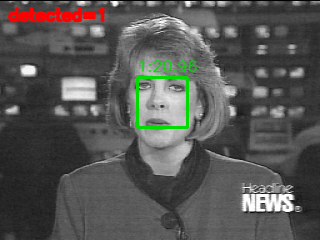
\includegraphics[width=\textwidth]{results/cmu_result_01_cnn2600.png}
        \\[2pt]{\small CMU 测试结果 1}
    \end{minipage}\hfill
    \begin{minipage}{0.48\textwidth}
        \centering
        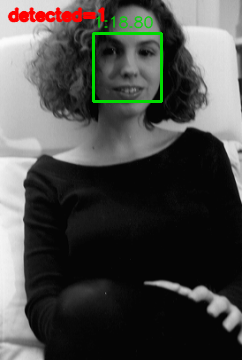
\includegraphics[width=\textwidth]{results/cmu_result_02_kaari2.png}
        \\[2pt]{\small CMU 测试结果 2}
    \end{minipage}
\end{figure}

\begin{figure}[H]
    \centering
    \begin{minipage}{0.48\textwidth}
        \centering
        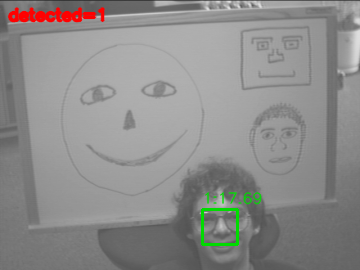
\includegraphics[width=\textwidth]{results/cmu_result_03_henry.png}
        \\[2pt]{\small CMU 测试结果 3}
    \end{minipage}\hfill
    \begin{minipage}{0.48\textwidth}
        \centering
        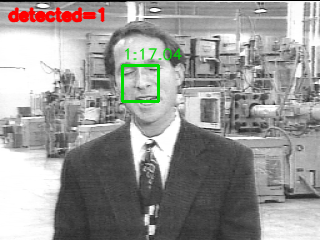
\includegraphics[width=\textwidth]{results/cmu_result_04_cnn2221.png}
        \\[2pt]{\small CMU 测试结果 4}
    \end{minipage}
\end{figure}

\begin{figure}[H]
    \centering
    \begin{minipage}{0.55\textwidth}
        \centering
        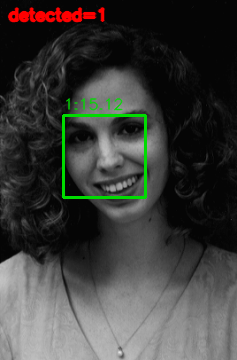
\includegraphics[width=\textwidth]{results/cmu_result_05_kaari1.png}
        \\[2pt]{\small CMU 测试结果 5}
    \end{minipage}
\end{figure}

为了更直观地分析分类器性能，实验绘制了测试分数分布图和 ROC 曲线。可以看到，人脸 patch 与非人脸 patch 的得分分布已经具有较明显分离，说明当前训练得到的级联分类器具有较好的二分类能力。

\begin{figure}[H]
    \centering
    \begin{minipage}{0.48\textwidth}
        \centering
        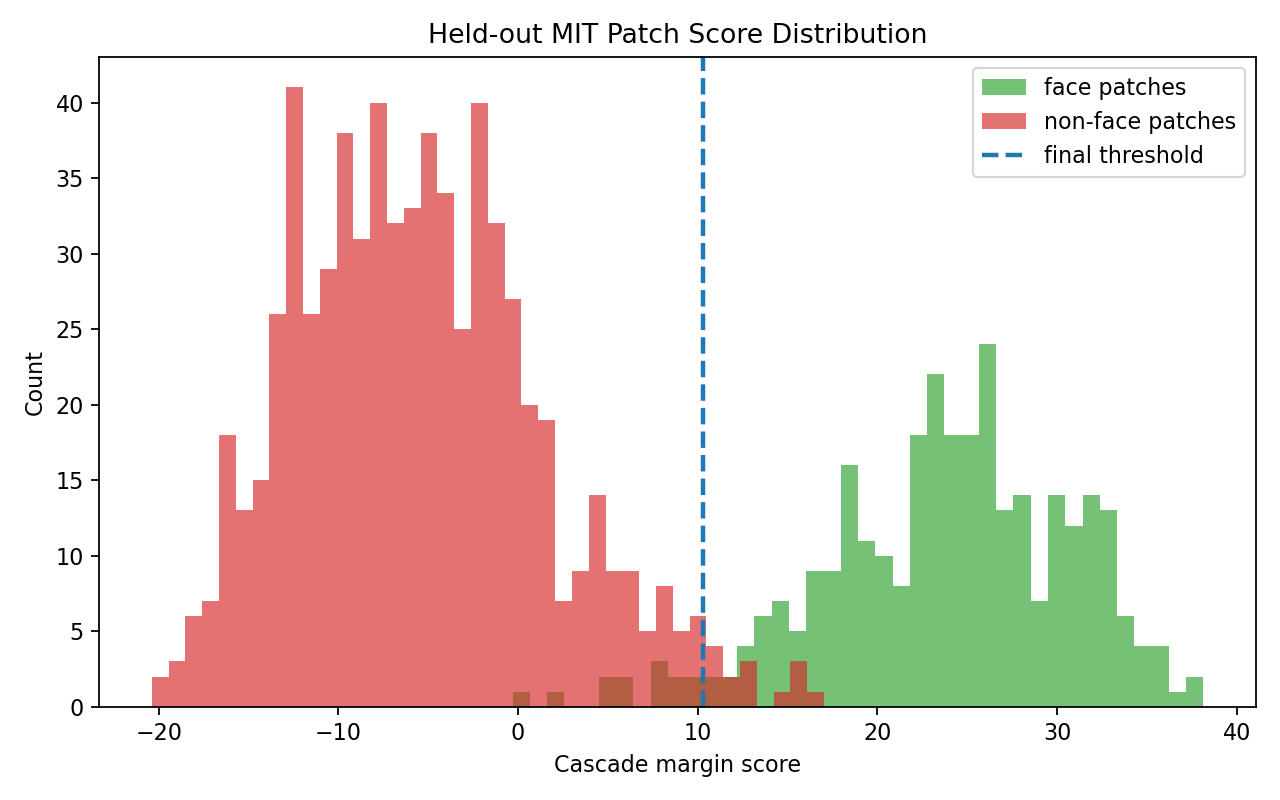
\includegraphics[width=\textwidth]{results/score_histogram.png}
        \\[2pt]{\small 测试分数分布图}
    \end{minipage}\hfill
    \begin{minipage}{0.48\textwidth}
        \centering
        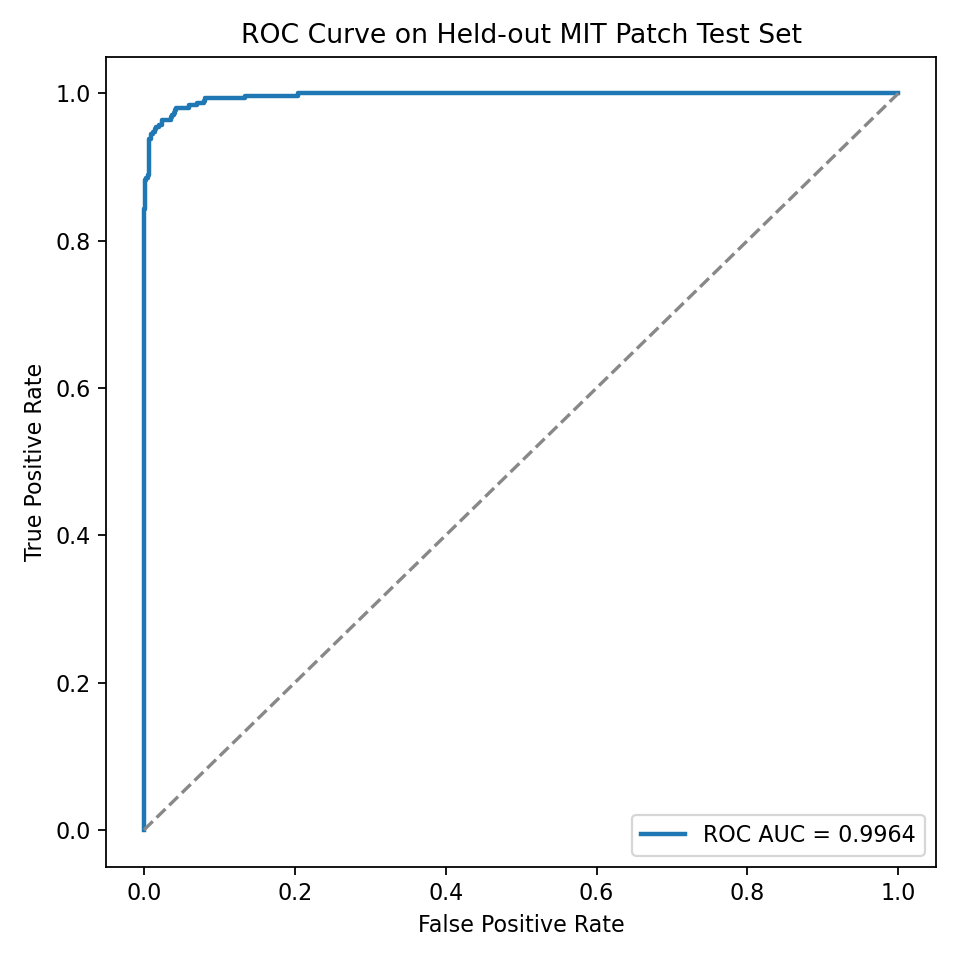
\includegraphics[width=\textwidth]{results/roc_curve.png}
        \\[2pt]{\small ROC 曲线}
    \end{minipage}
\end{figure}

\begin{figure}[H]
    \centering
    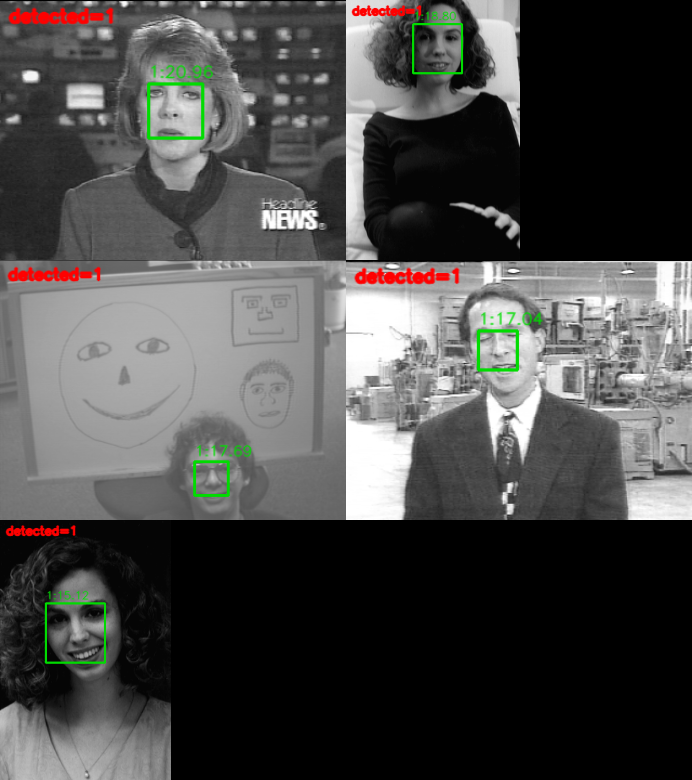
\includegraphics[width=0.92\textwidth]{results/summary.png}
    \\[4pt]{\small 5 张外部测试图像检测结果汇总}
\end{figure}

\item \textbf{实验小结}

本实验按照“Haar 特征 + 积分图 + AdaBoost + 级联”的经典流程实现了一个自训练的人脸检测器。训练阶段以 MIT face/nonface patch 数据集为基础，先计算积分图，再提取 Haar 特征，通过 AdaBoost 逐级训练强分类器，并将多个强分类器串联形成级联结构。测试阶段则将训练好的模型应用到独立的 CMU frontal\_images 数据集上，采用多尺度滑窗方式完成整图中的人脸检测。

从实验结果可以看出，模型在 MIT 独立测试集上的 patch 分类指标较好，说明它能够有效区分人脸 patch 与非人脸 patch；同时，在 CMU 外部测试图像上也能够完成较稳定的正面人脸检测。为了减少结果图中出现大量空框，本实验在最终阈值调节时优先控制假阳性率，并在后处理阶段加入了重叠支持过滤，因此当前结果图中的误检数量较前期版本明显下降，整体观感更适合作业展示。

需要说明的是，patch 级分类和整图滑窗检测之间仍然存在难度差异。即使 patch 测试上的假阳性率已经较低，整图检测时由于候选窗口数量较多，仍可能出现少量误检。因此，若继续改进，可以考虑进一步增加困难负样本挖掘、引入更细的多尺度搜索策略，或者使用更强的后处理方法来进一步提升整图检测效果。

\end{enumerate}

\end{document}
